
\documentclass{article}
\pagestyle{plain}
\usepackage[protrusion=true,expansion=true]{microtype}
\usepackage{graphicx}
\usepackage{wrapfig}
\usepackage{mathpazo}
\usepackage{csquotes}
\usepackage{indentfirst}
\usepackage{graphicx, wrapfig, mathpazo, csquotes, float, tcolorbox, amsmath, amssymb, tikz, subcaption}
\newcommand\tab[1][1cm]{\hspace*{#1}}

\begin{document}
\setlength\parindent{24pt}
\title{\textbf{Audio Ember}}
\author{\textsc{Robert Gonzalez, Kevin Williams and Michael Woodham}}
\date{08/02/2017}
\maketitle


\section*{Application Details}
The goal of the Application was to provide a service which Billboard is not currently providing:
data amalgamation and illustration of songs as they progress through charts, as well as a definitive answer to which songs have been the best in certain categories.
This was accomplished by assigning each song a point value.
Points are the accumulation of ranks brought about by our formula which determines the total points that the song has generated across all weeks up to the current week. 
Our formula is the following, 101 - rank of song on chart. 
For example, a song which was ranked 22 on the Hot-100 chart will have the value of 79 in the hot 100 chart.
As of current our app implements the Dates from January 1, 2016 to July 22, 2017 but we do intend to expand this time period in future updates.
\\ \tab Our target audience is probably going to be millennials given that our target data is such a small chunk of years, but in future updates our target audience will be member of all age brackets who love music.

\section*{Related Apps vs Our Application}
As far as how to format this section we considered a few different implementations.
Either to go over a few different apps on the Google-Play store and go over each of their pit falls, or to sum them all up into one category. 
In an attempt to void redundancies as all for their pit-falls are the same, we have opted to go for a summary. 
We do concede that as of current standing other applications do look better than ours (Billboard Radio, Spotify, Mueso) all of which provide stream and listening options,
but as far as data goes we can not find another application which succeeds in this area.
\\ \tab As it currently stands, chart apps appear to care about this weeks charts and standings in the music industry, but for previous charts, they all fail to notice them. 
We believe that the reason for this is that there is no perceived demand for a publicly accessible database reporting chart progression of music.
We beg to differ and contract this notion as we find this field fascinating and do believe that others feel the same.
We on the other hand do not believe that billboard would wish for the public to see how songs do fair on charts overtime as it does reveal some intricacies and inconsistencies within the industry,
but that is not for us to decide, but rather for the viewer. 
The data does tend to speak for itself.

\section*{Development Time line}
\subsection*{Original Concept Design}
As can be seen in the two figures below, our original design was to have the user search for Songs or Artists in the Database or have a guided menu by genre, month, or year. This was scraped for the reasons of time and simplicity. We felt that this page would overwhelm users with too much information accessible at the start. 
\begin{figure}[H]
  \centering
  \begin{minipage}{.5\textwidth}
    \centering
    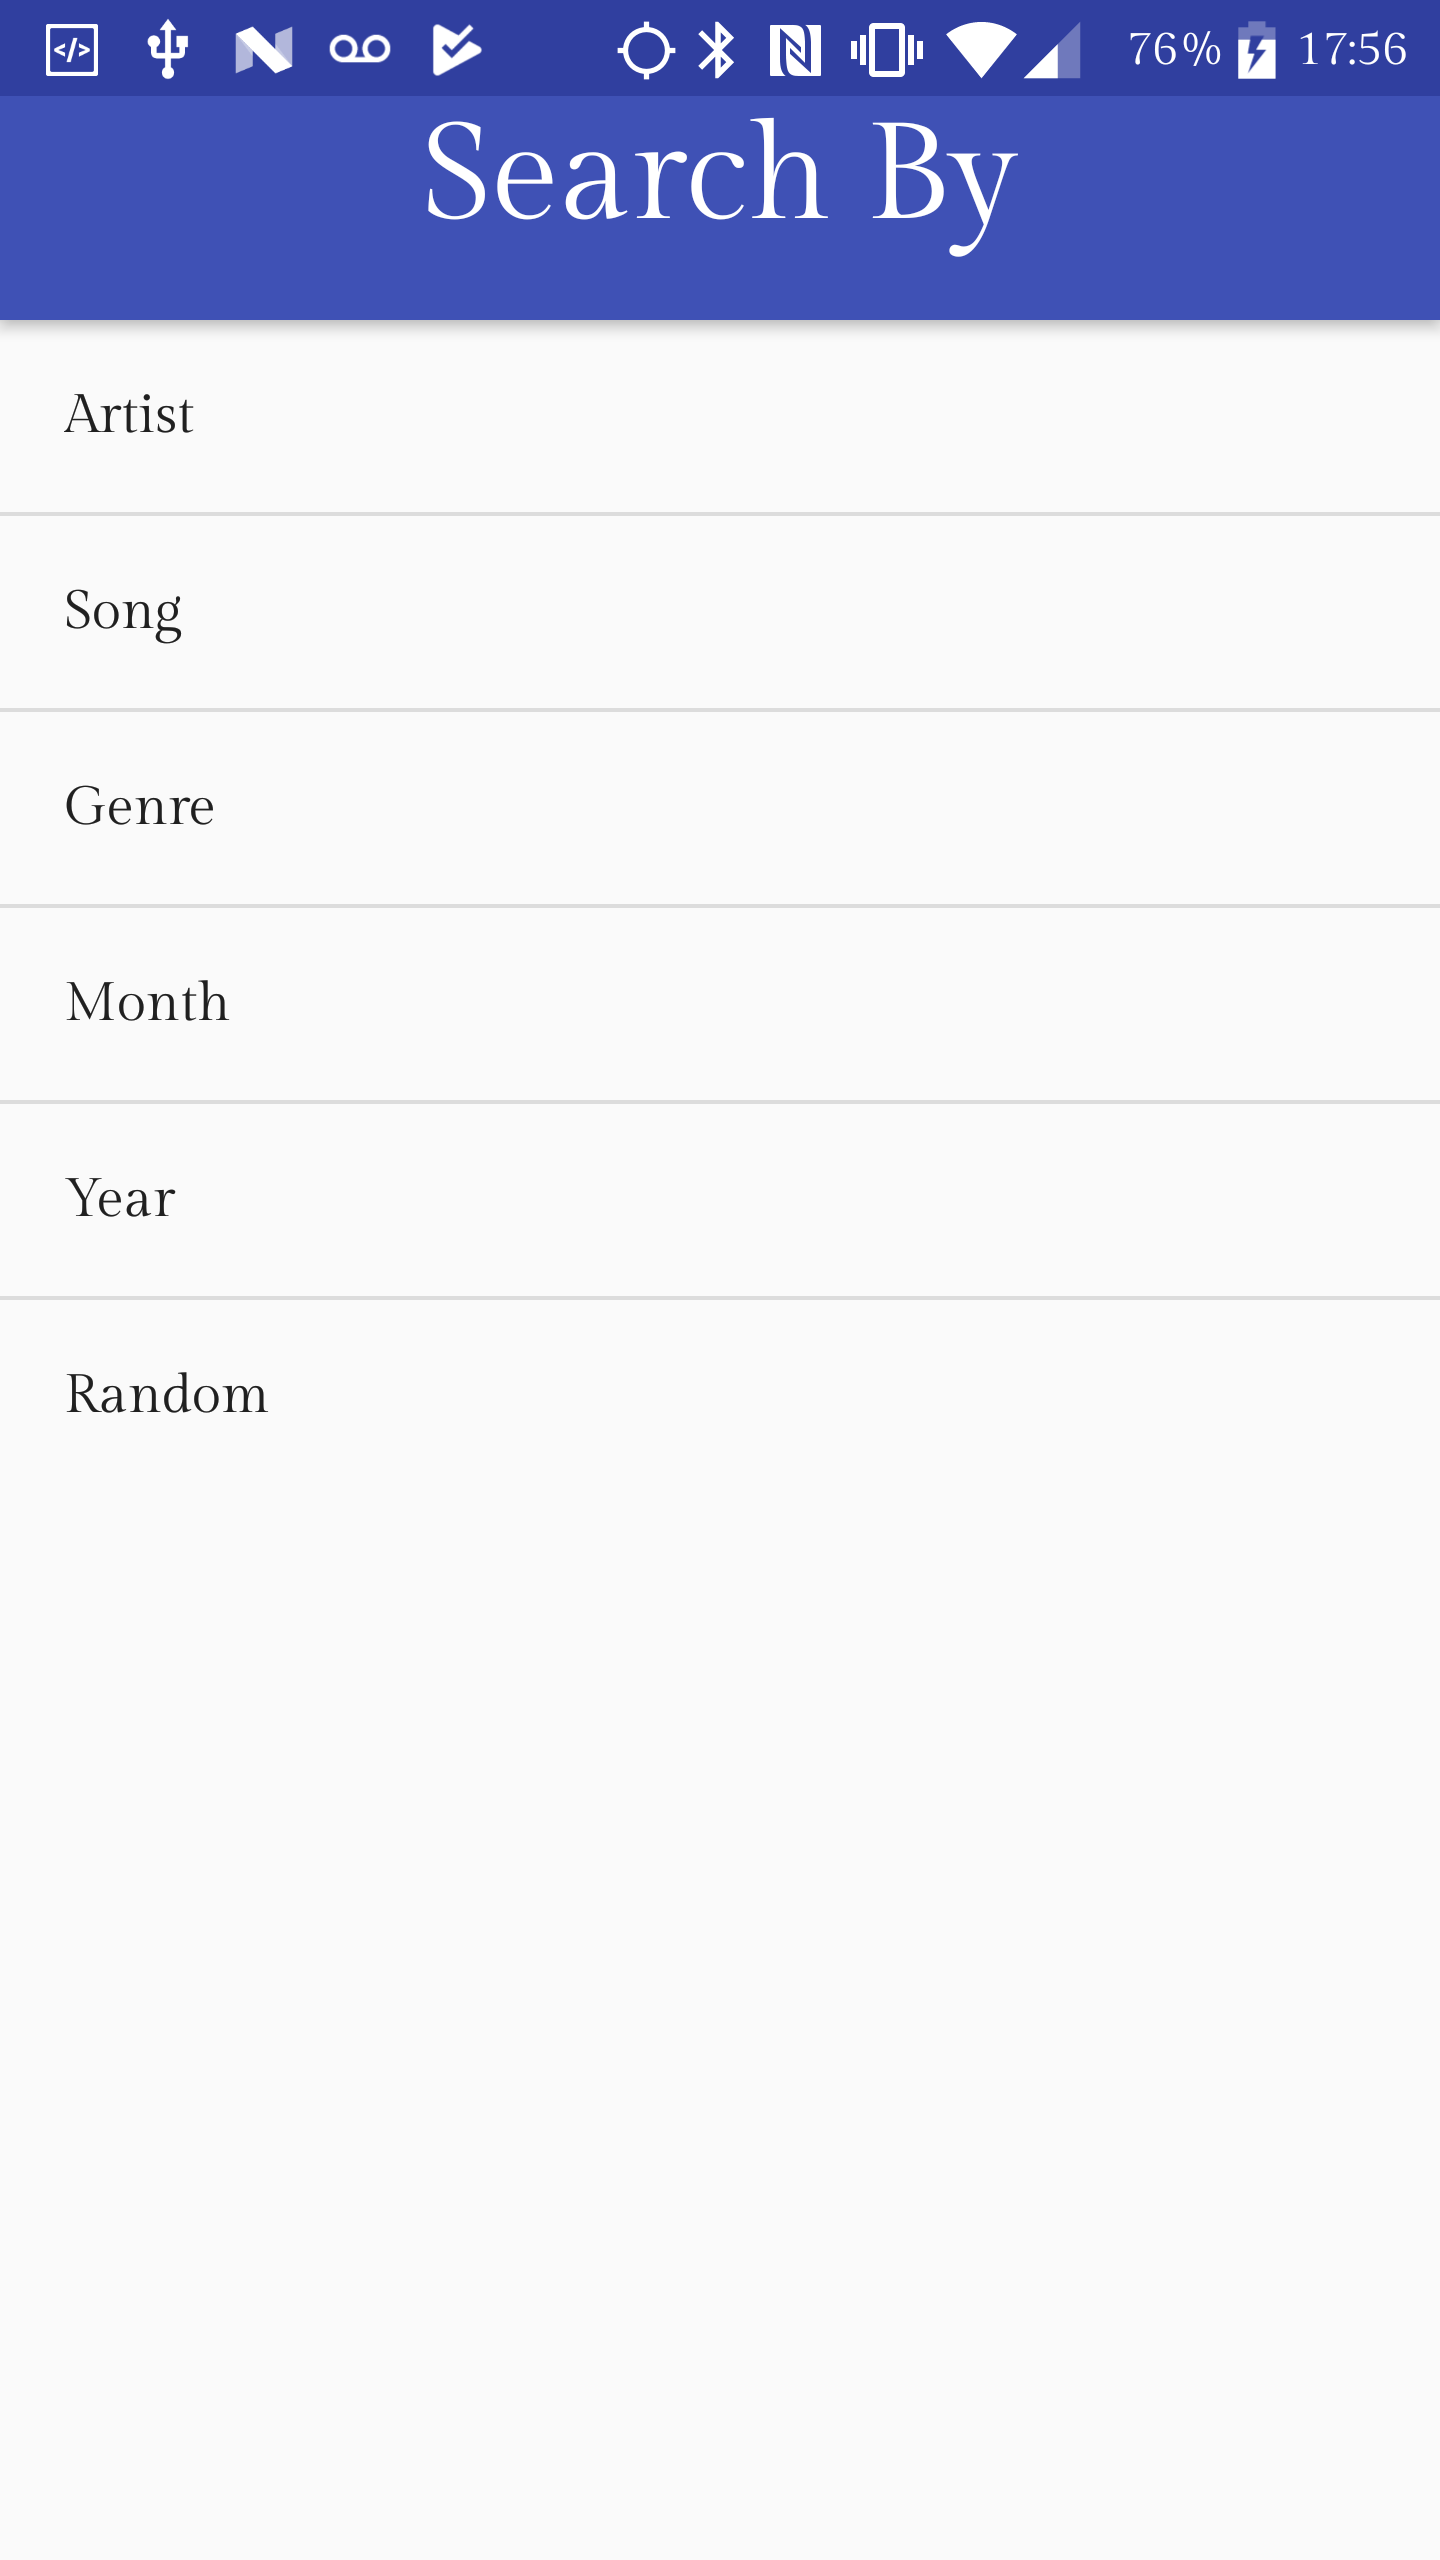
\includegraphics[width=0.9\textwidth]{Original_Home_Page.png}
    \caption{Month Selector}
    \label{label}
  \end{minipage}%
  \begin{minipage}{.5\textwidth}
    \centering
    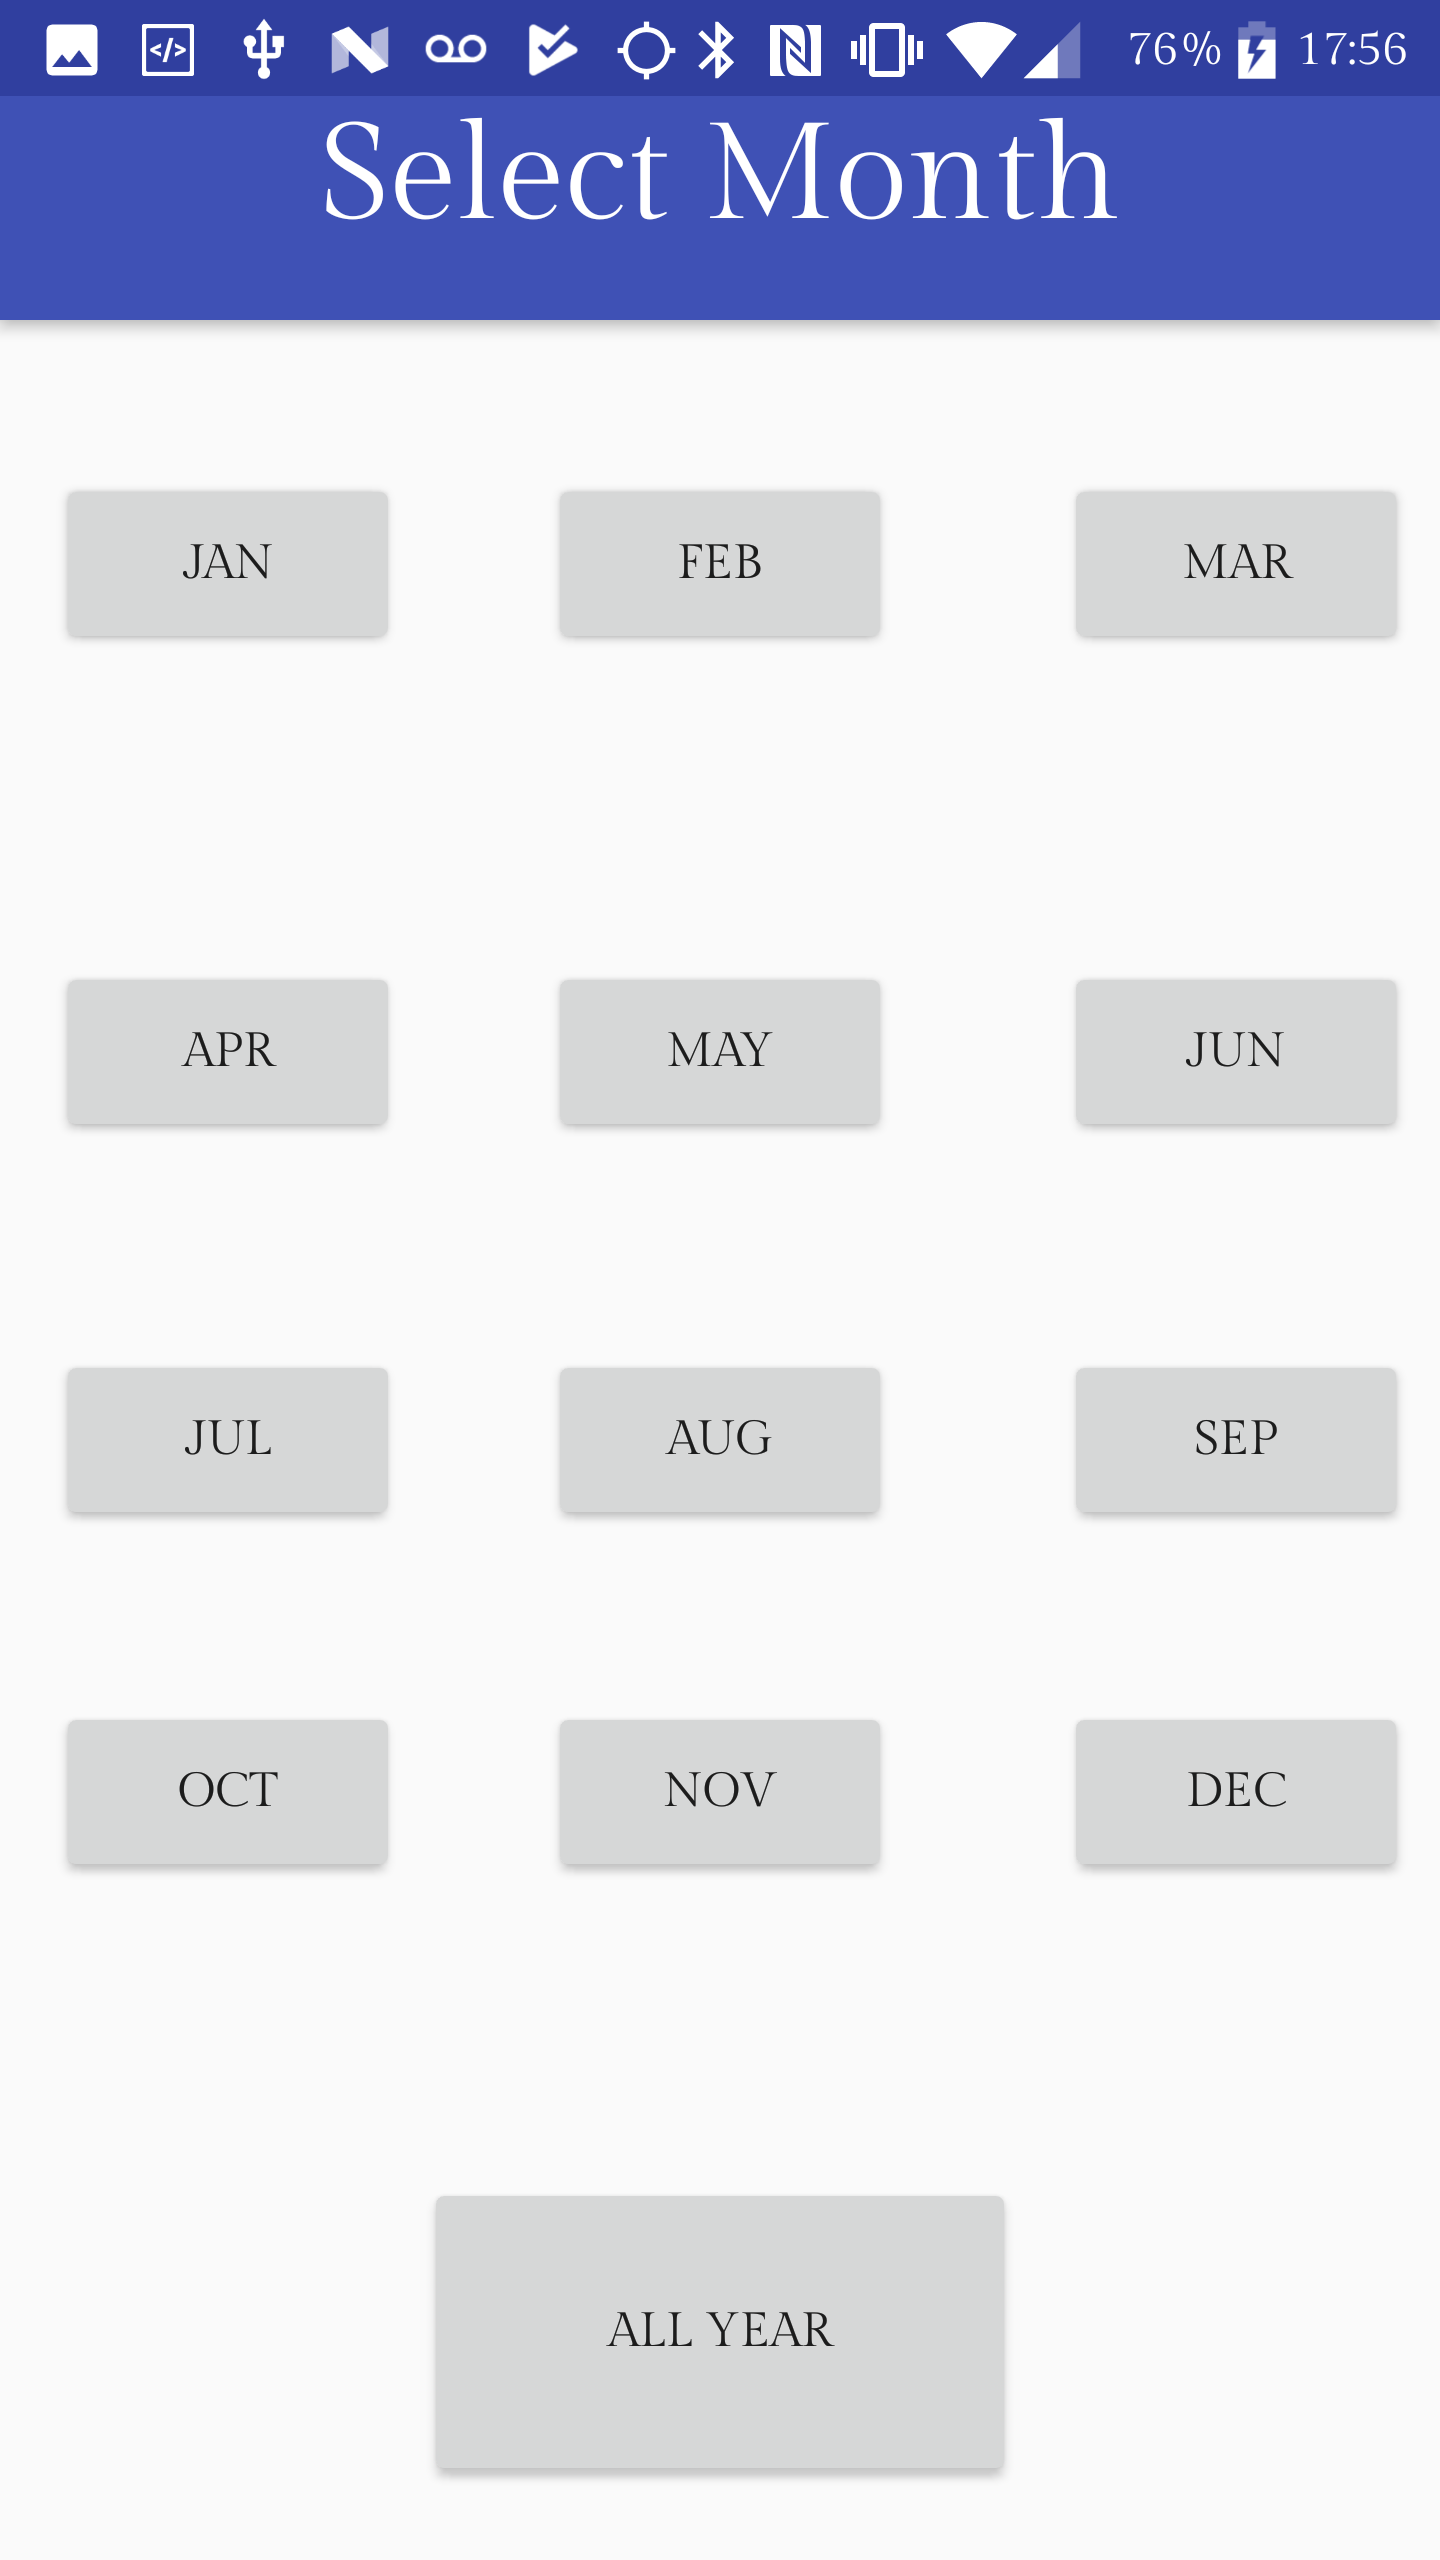
\includegraphics[width=0.9\textwidth]{Original_Month_Selector.png}
    \caption{Search Bar}
    \label{fig:ER}
  \end{minipage}
\end{figure}
Here you can see our original artist page. This was later revised to match the color format of our project, but the general idea did remain the same.
\begin{figure}[H]
  \begin{center}
    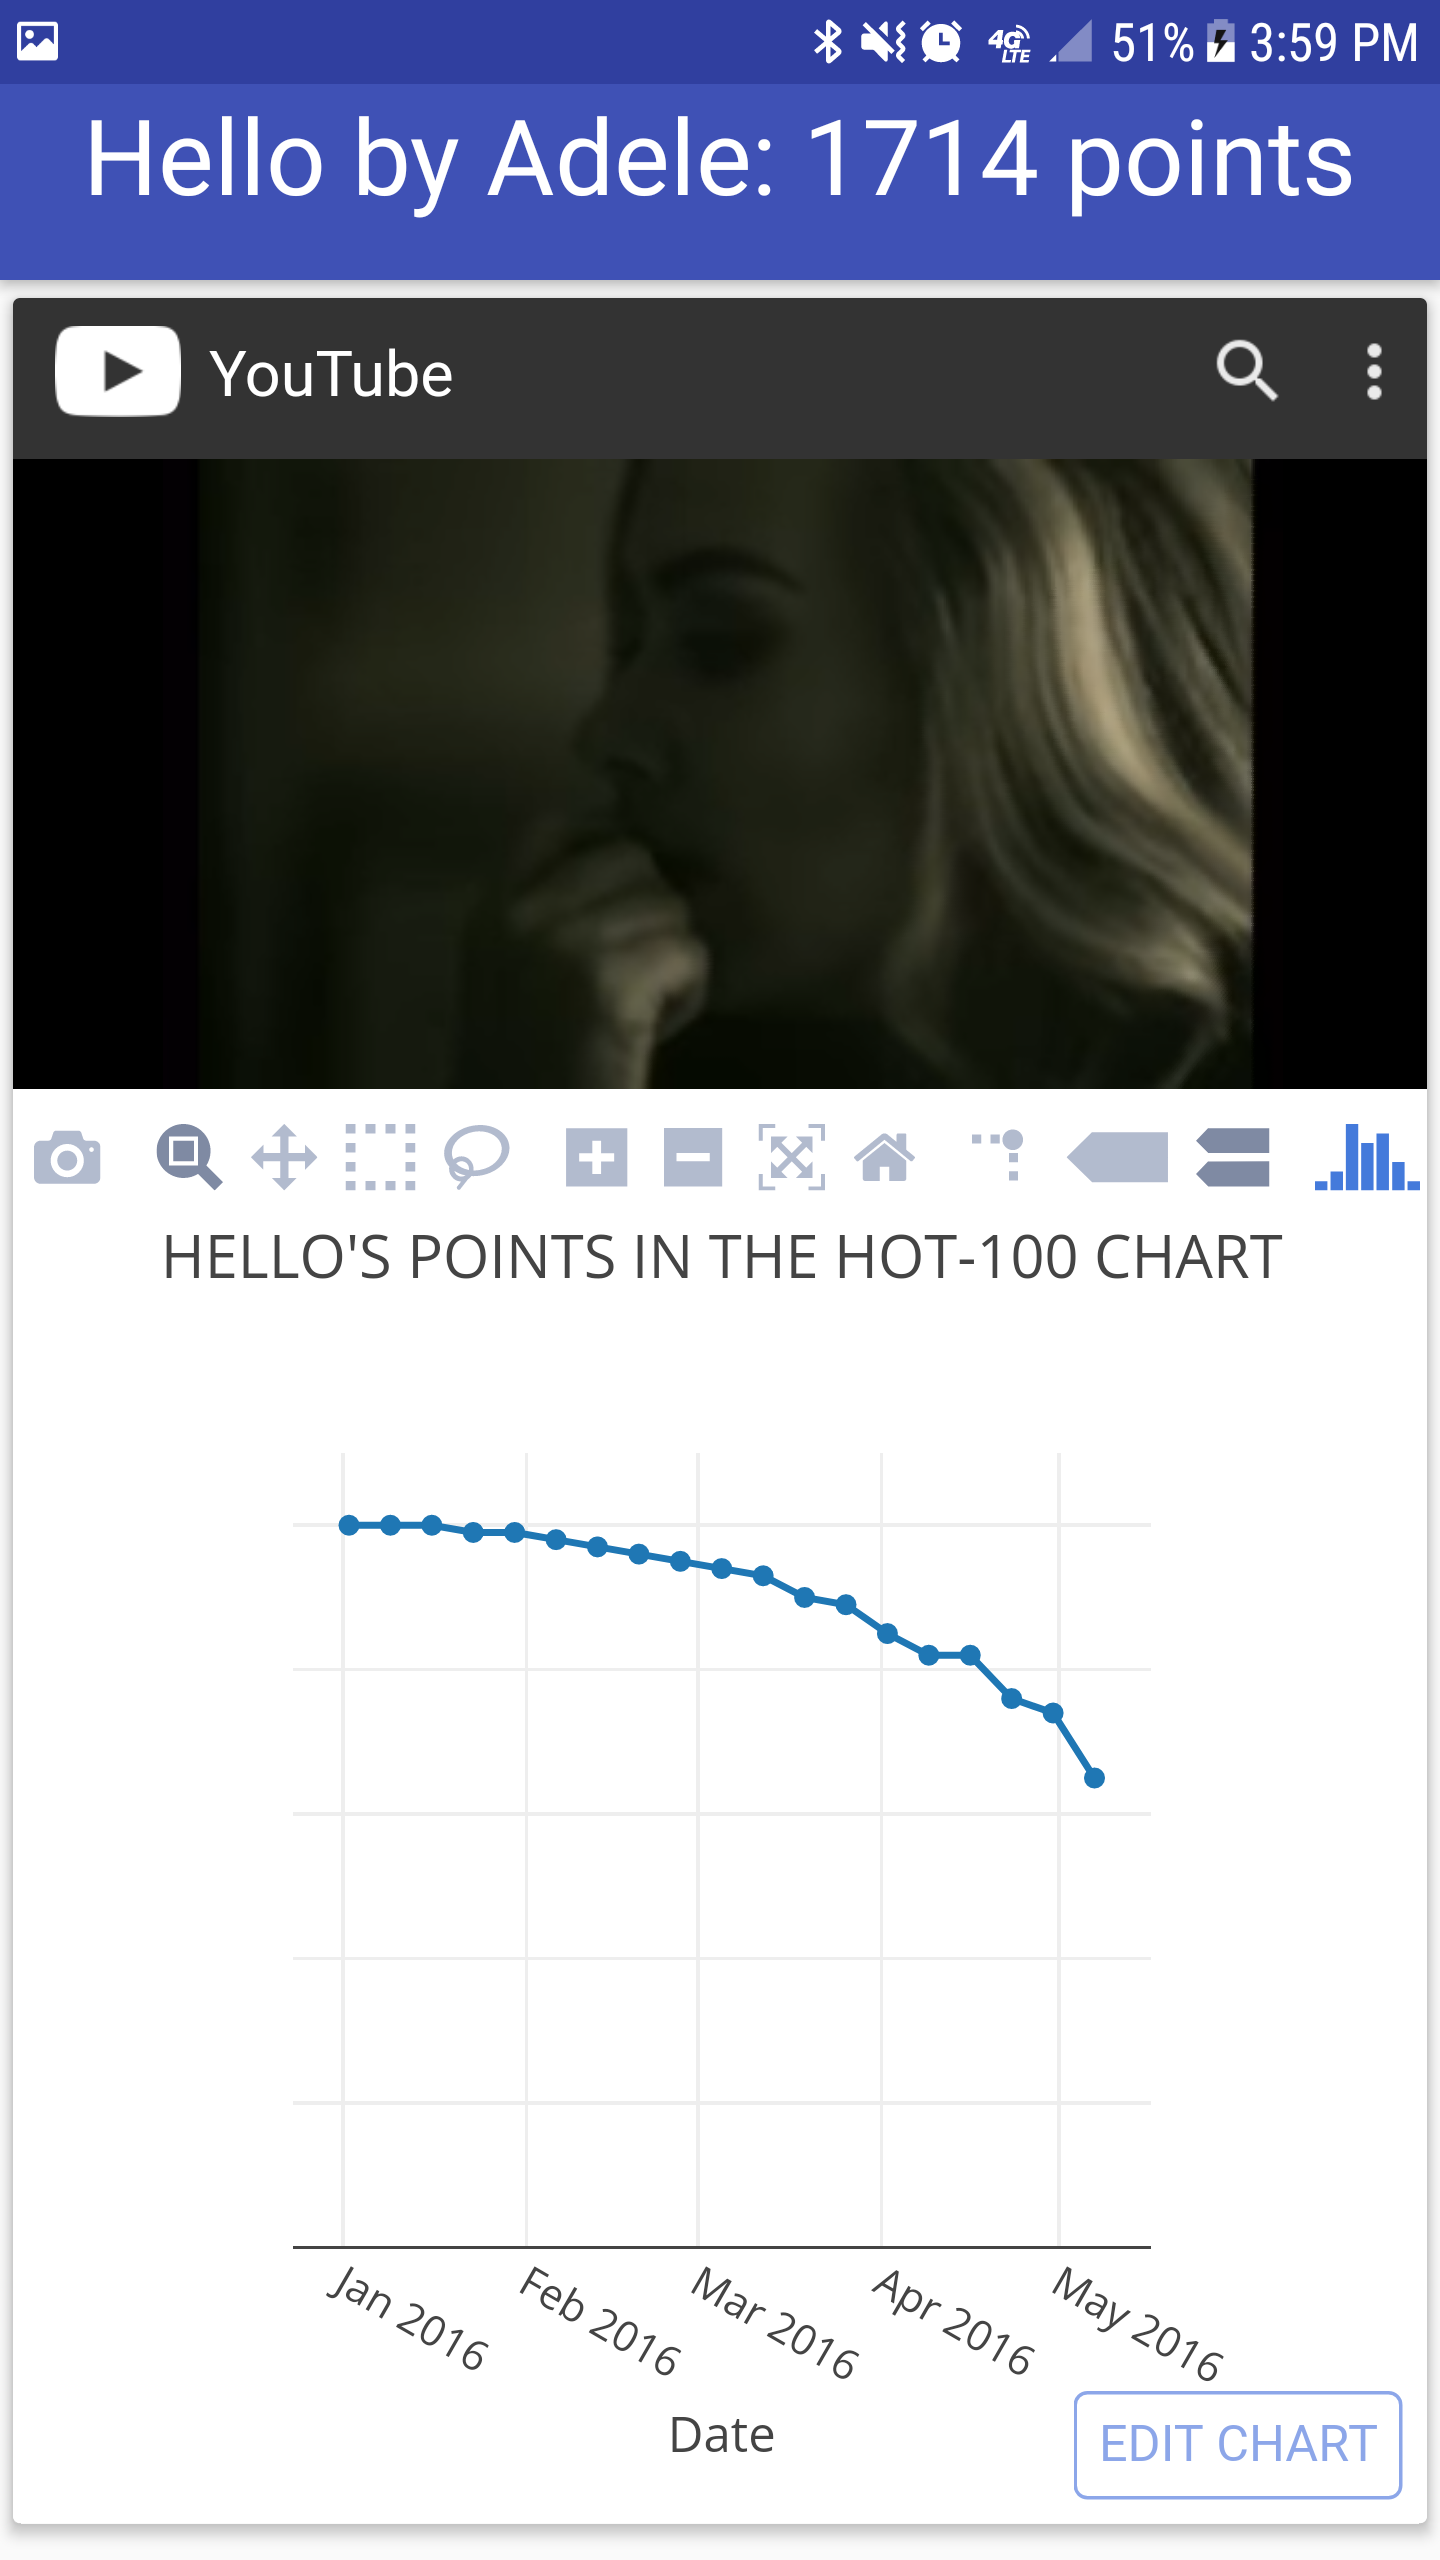
\includegraphics[width=0.45\textwidth]{original_song_graph.png}
    \caption{Original Song Page}
    \label{fig:ER}
  \end{center}
\end{figure}
Not shown is the second revision before we settled on our final design. In this revision There was a bottom bar similar to our final design. This bar was dynamic and would change given the user's position in the application either having 3, 4, or just two options. This design was scrapped for two reasons. Firstly, our artist integration was unable to be finalized in the project so that eliminated the need for a lot of our options. Secondly, with artist integration gone, most of our implementation was deemed to be redundant, resulting in our final design being built. 
\\ \\ \tab The third and final revision is shown below. We opted for a simple design of three buttons. Gone is the search function, gone is the date function, and what is left is a simple list from the top songs in a specific genre as determined by the user in the second option of the bottom bar. The third option is the video and graph generation for the specific song. While it is a downgrade from our original concept, we are happy with the results, and will be implementing the final product in future generations. 
\begin{figure}[H]
  \centering
  \begin{minipage}{.5\textwidth}
    \centering
    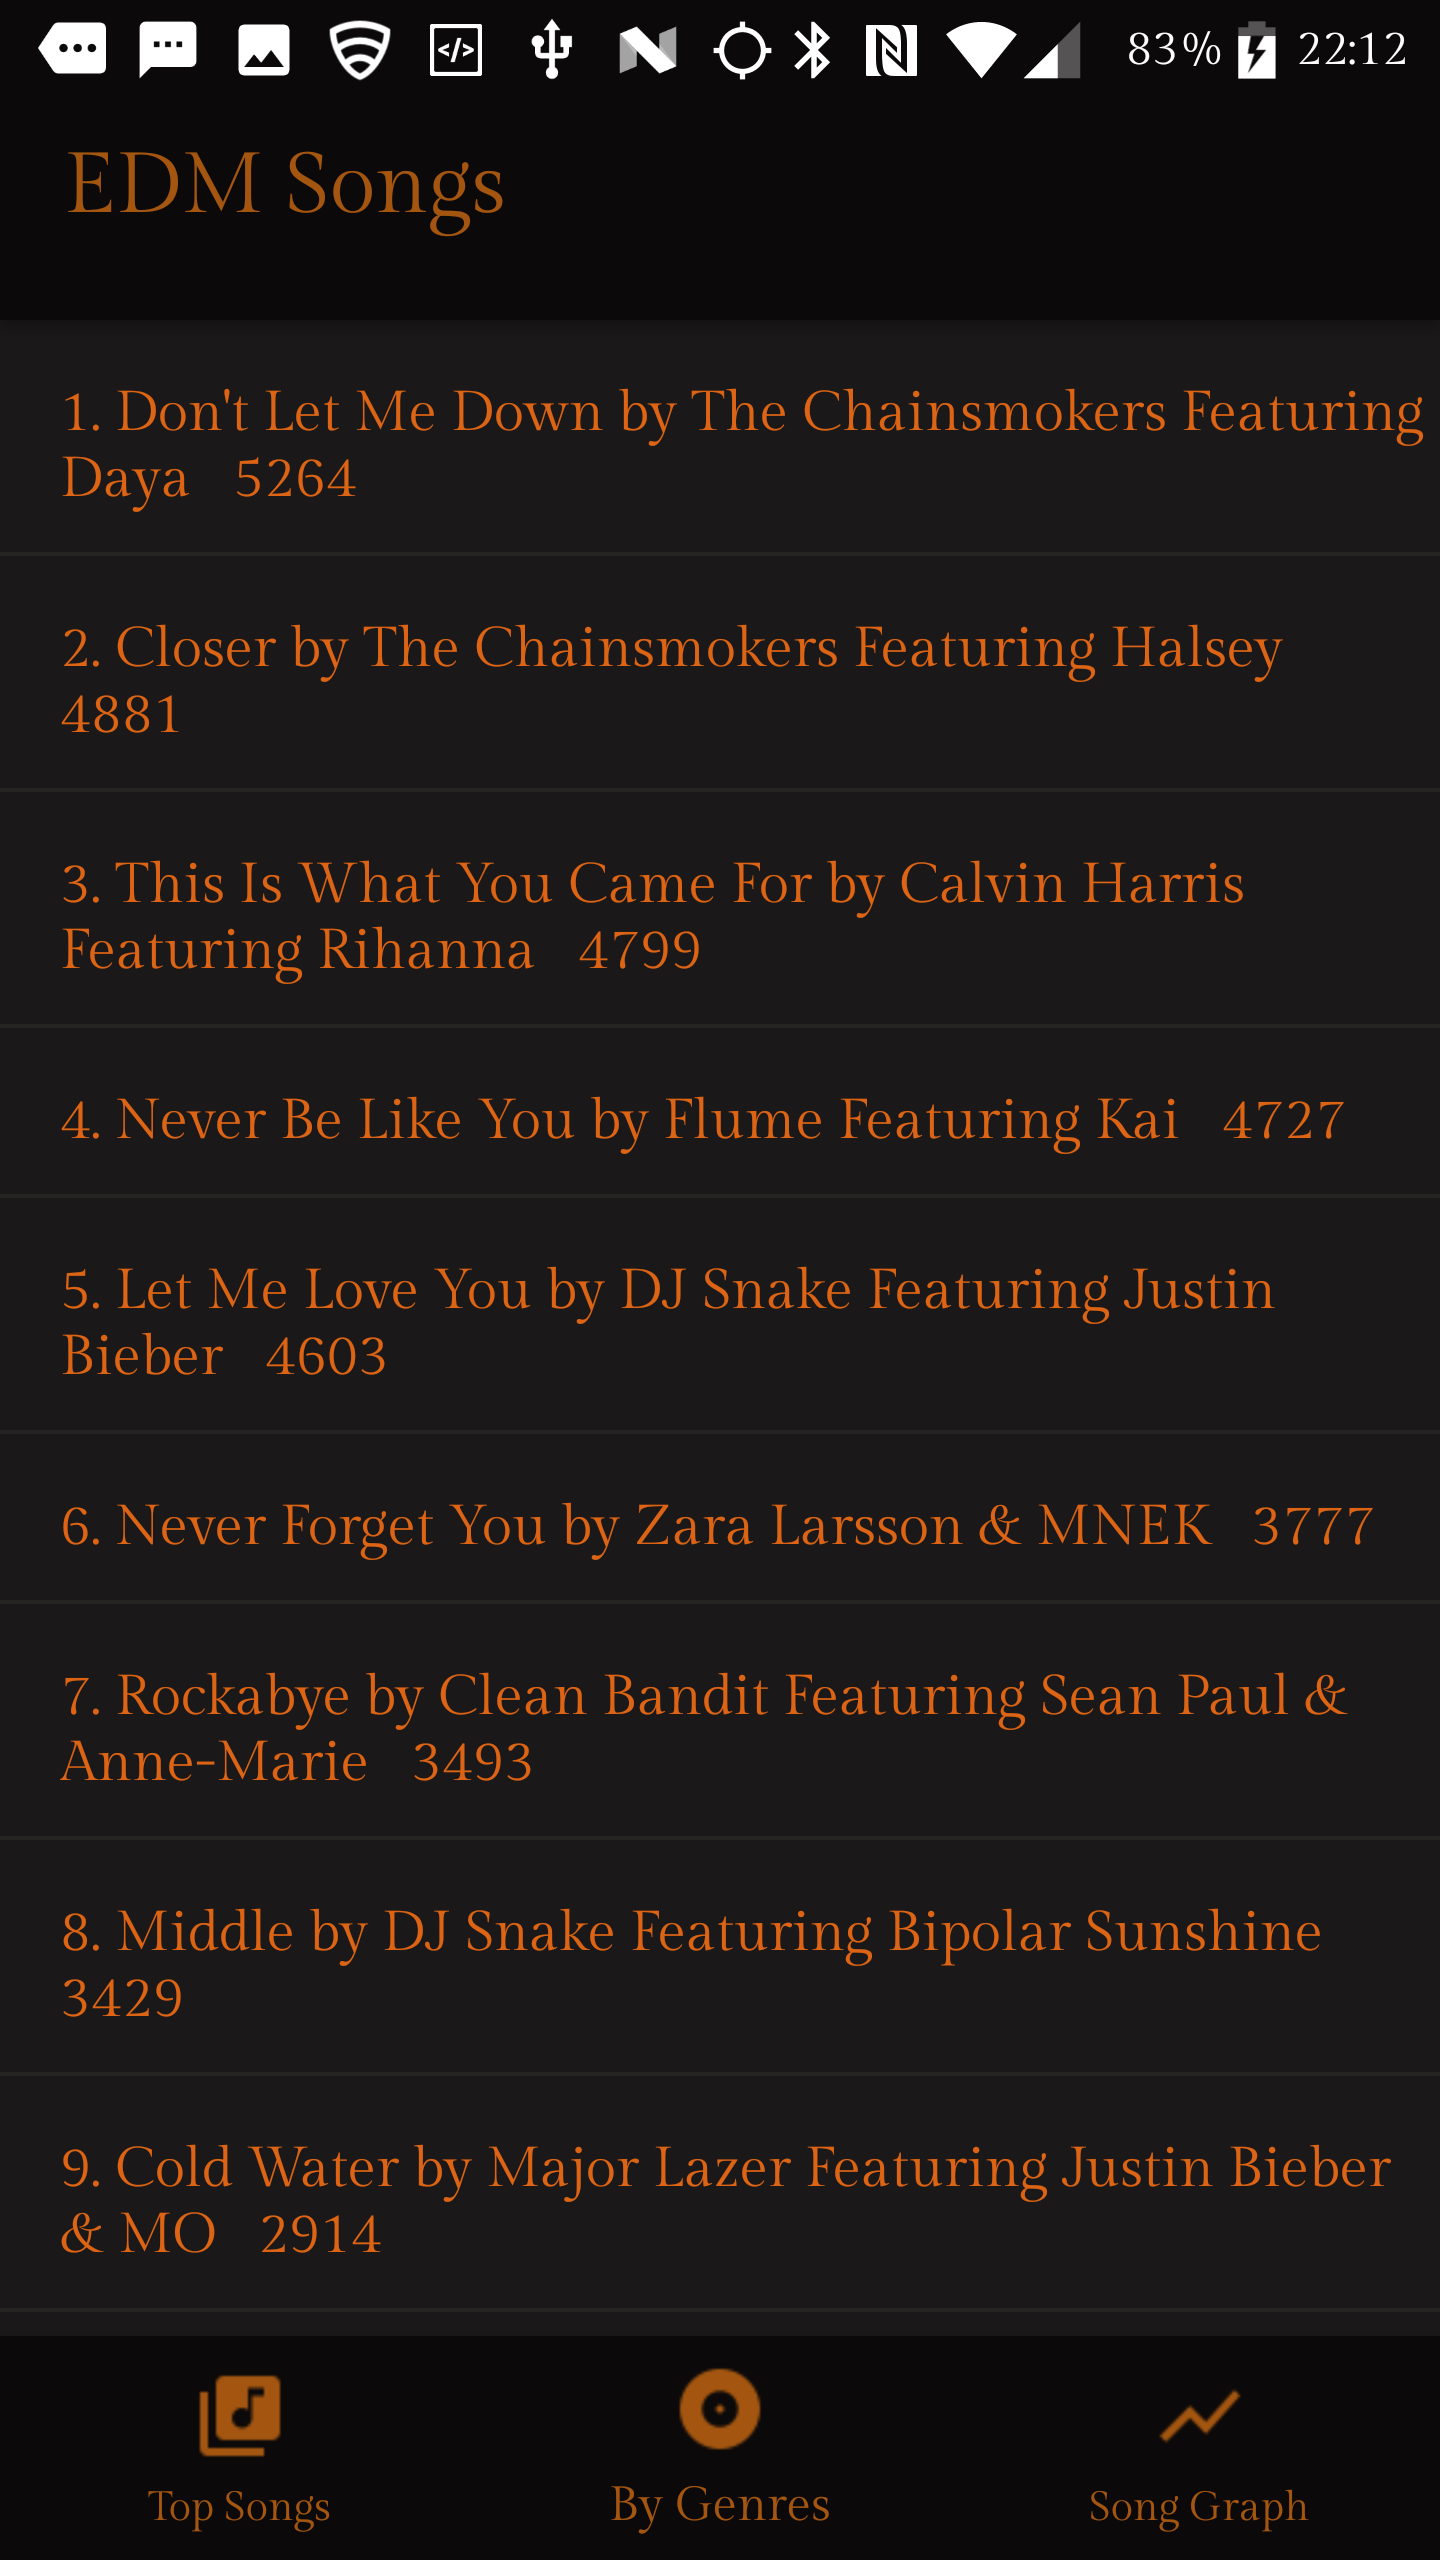
\includegraphics[width=0.75\textwidth]{EDMTop.png}
    \caption{Top EDM Songs}
    \label{label}
  \end{minipage}%
  \begin{minipage}{.5\textwidth}
    \centering
    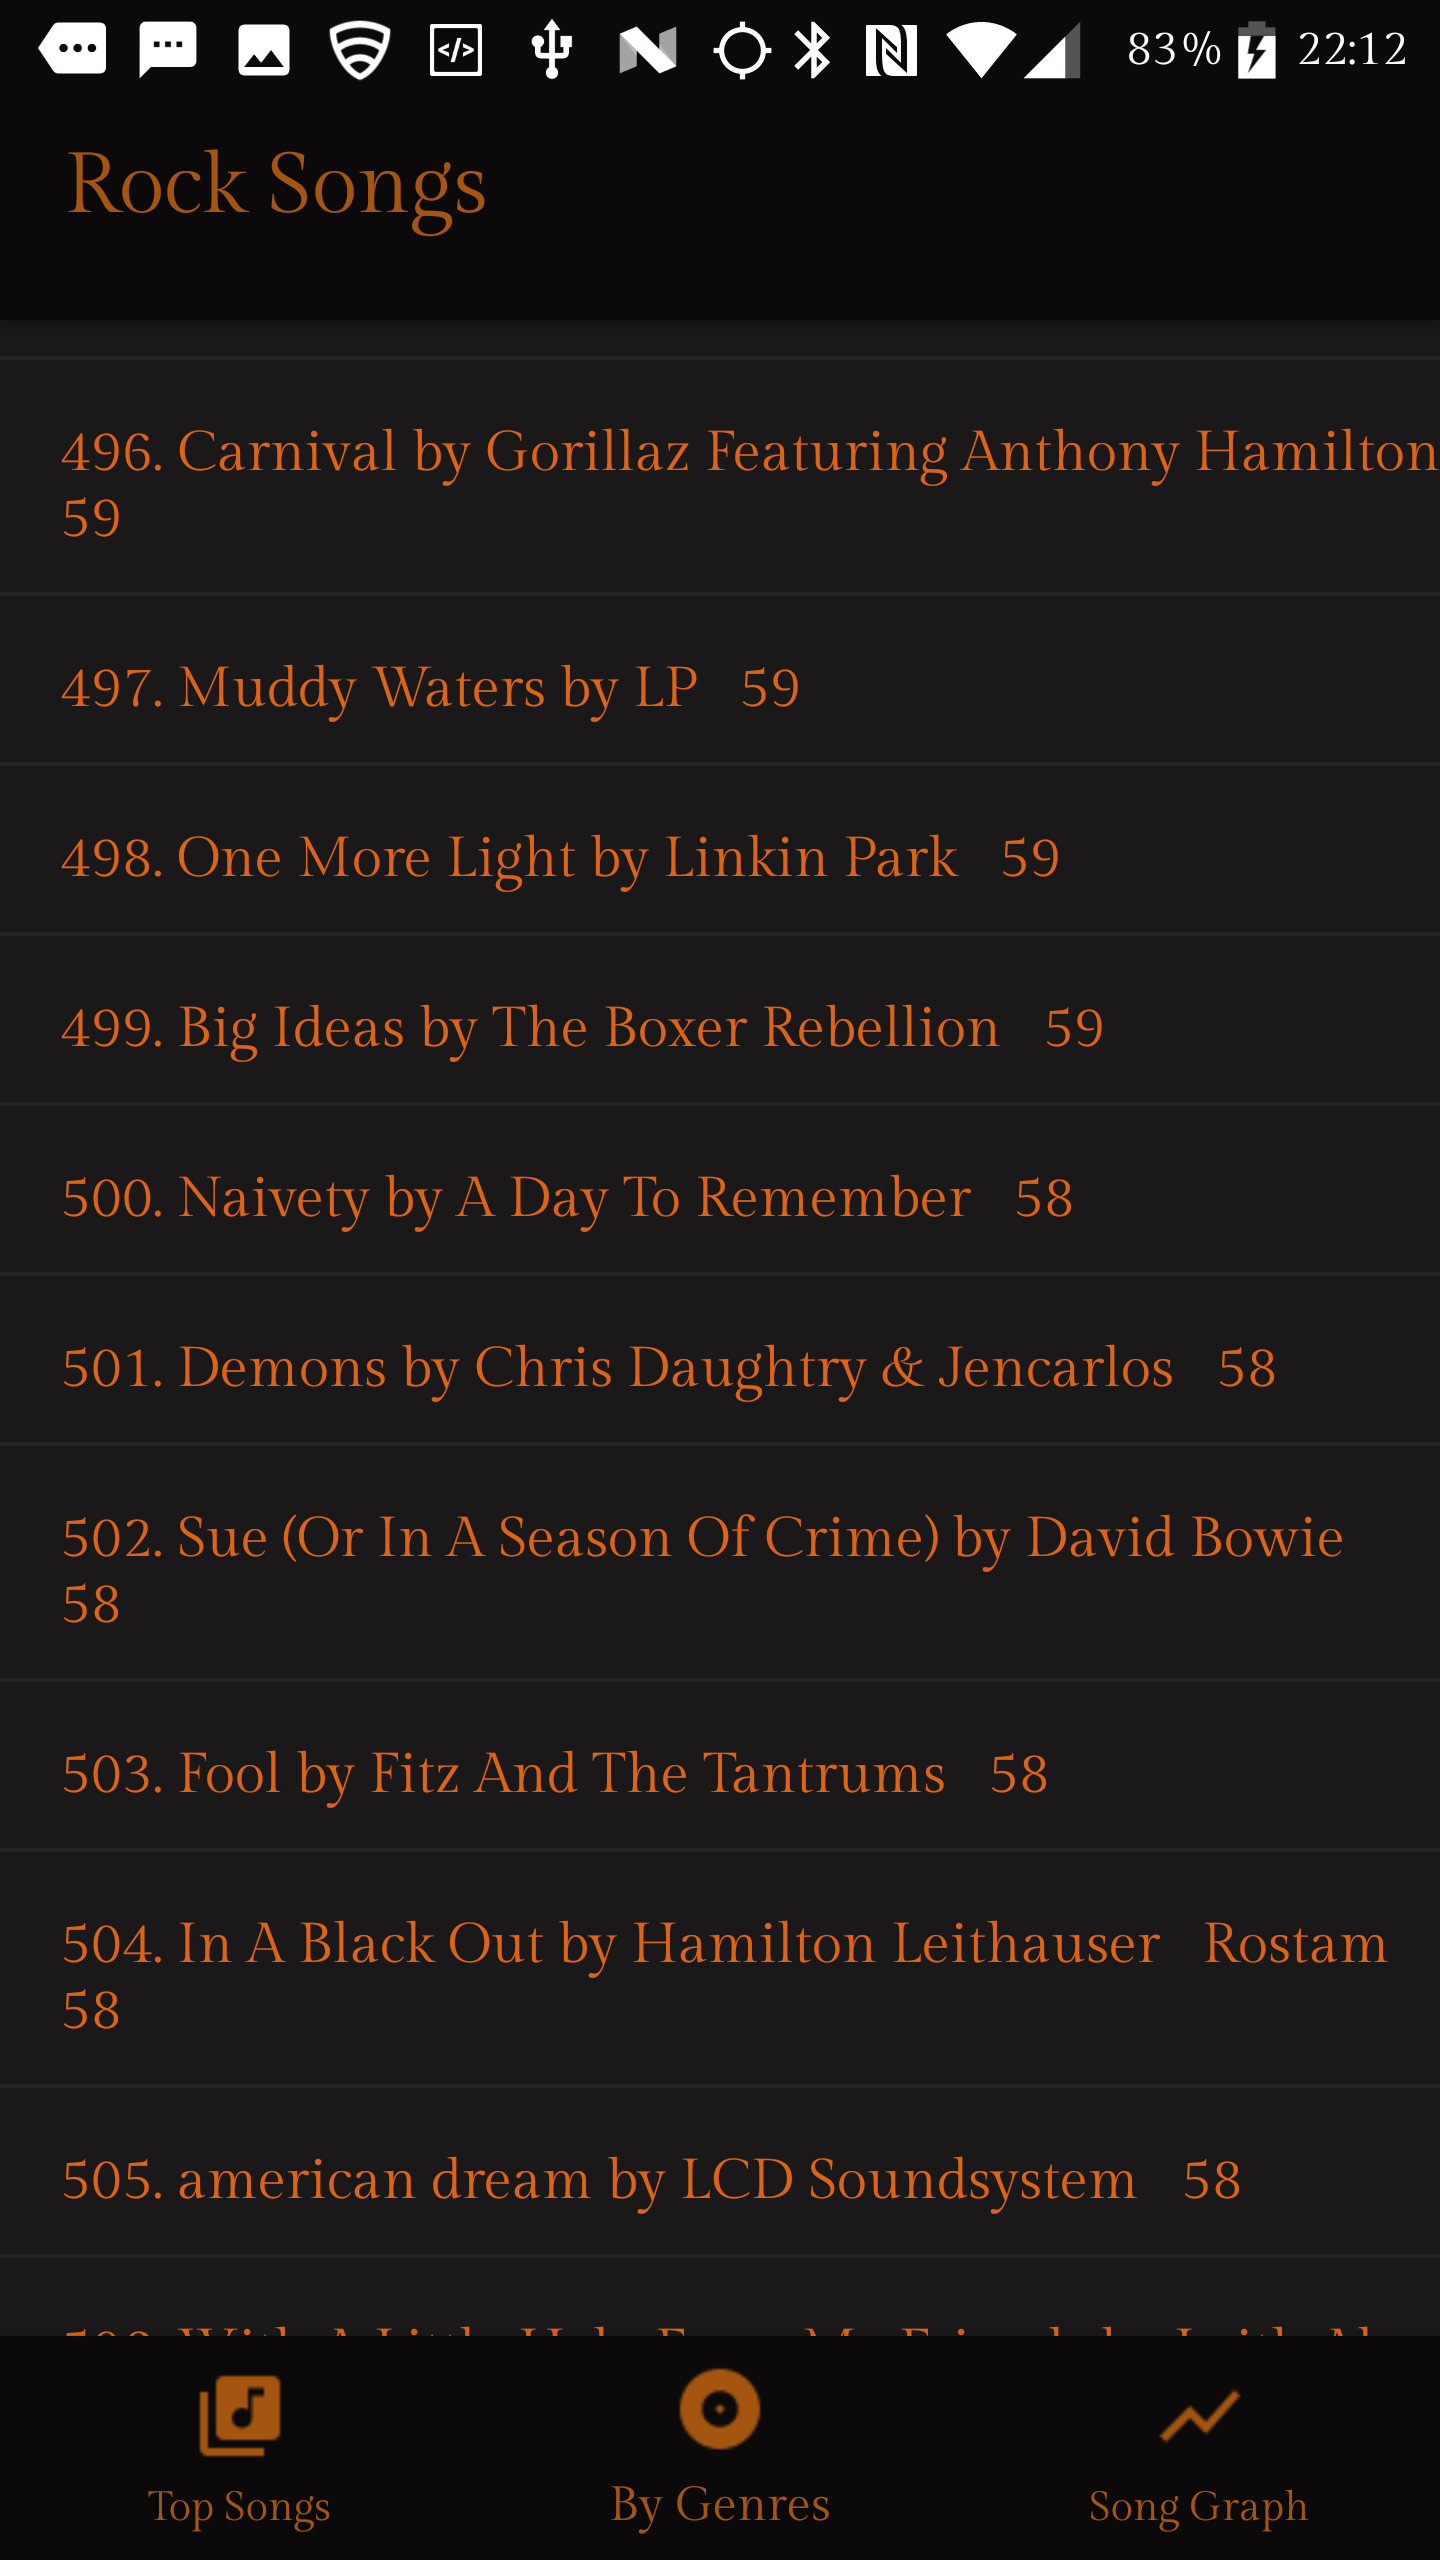
\includegraphics[width=0.75\textwidth]{RockList.png}
    \caption{Rock Songs Lower}
    \label{fig:ER}
  \end{minipage}
\end{figure}
\begin{figure}[H]
  \centering
  \begin{minipage}{.5\textwidth}
    \centering
    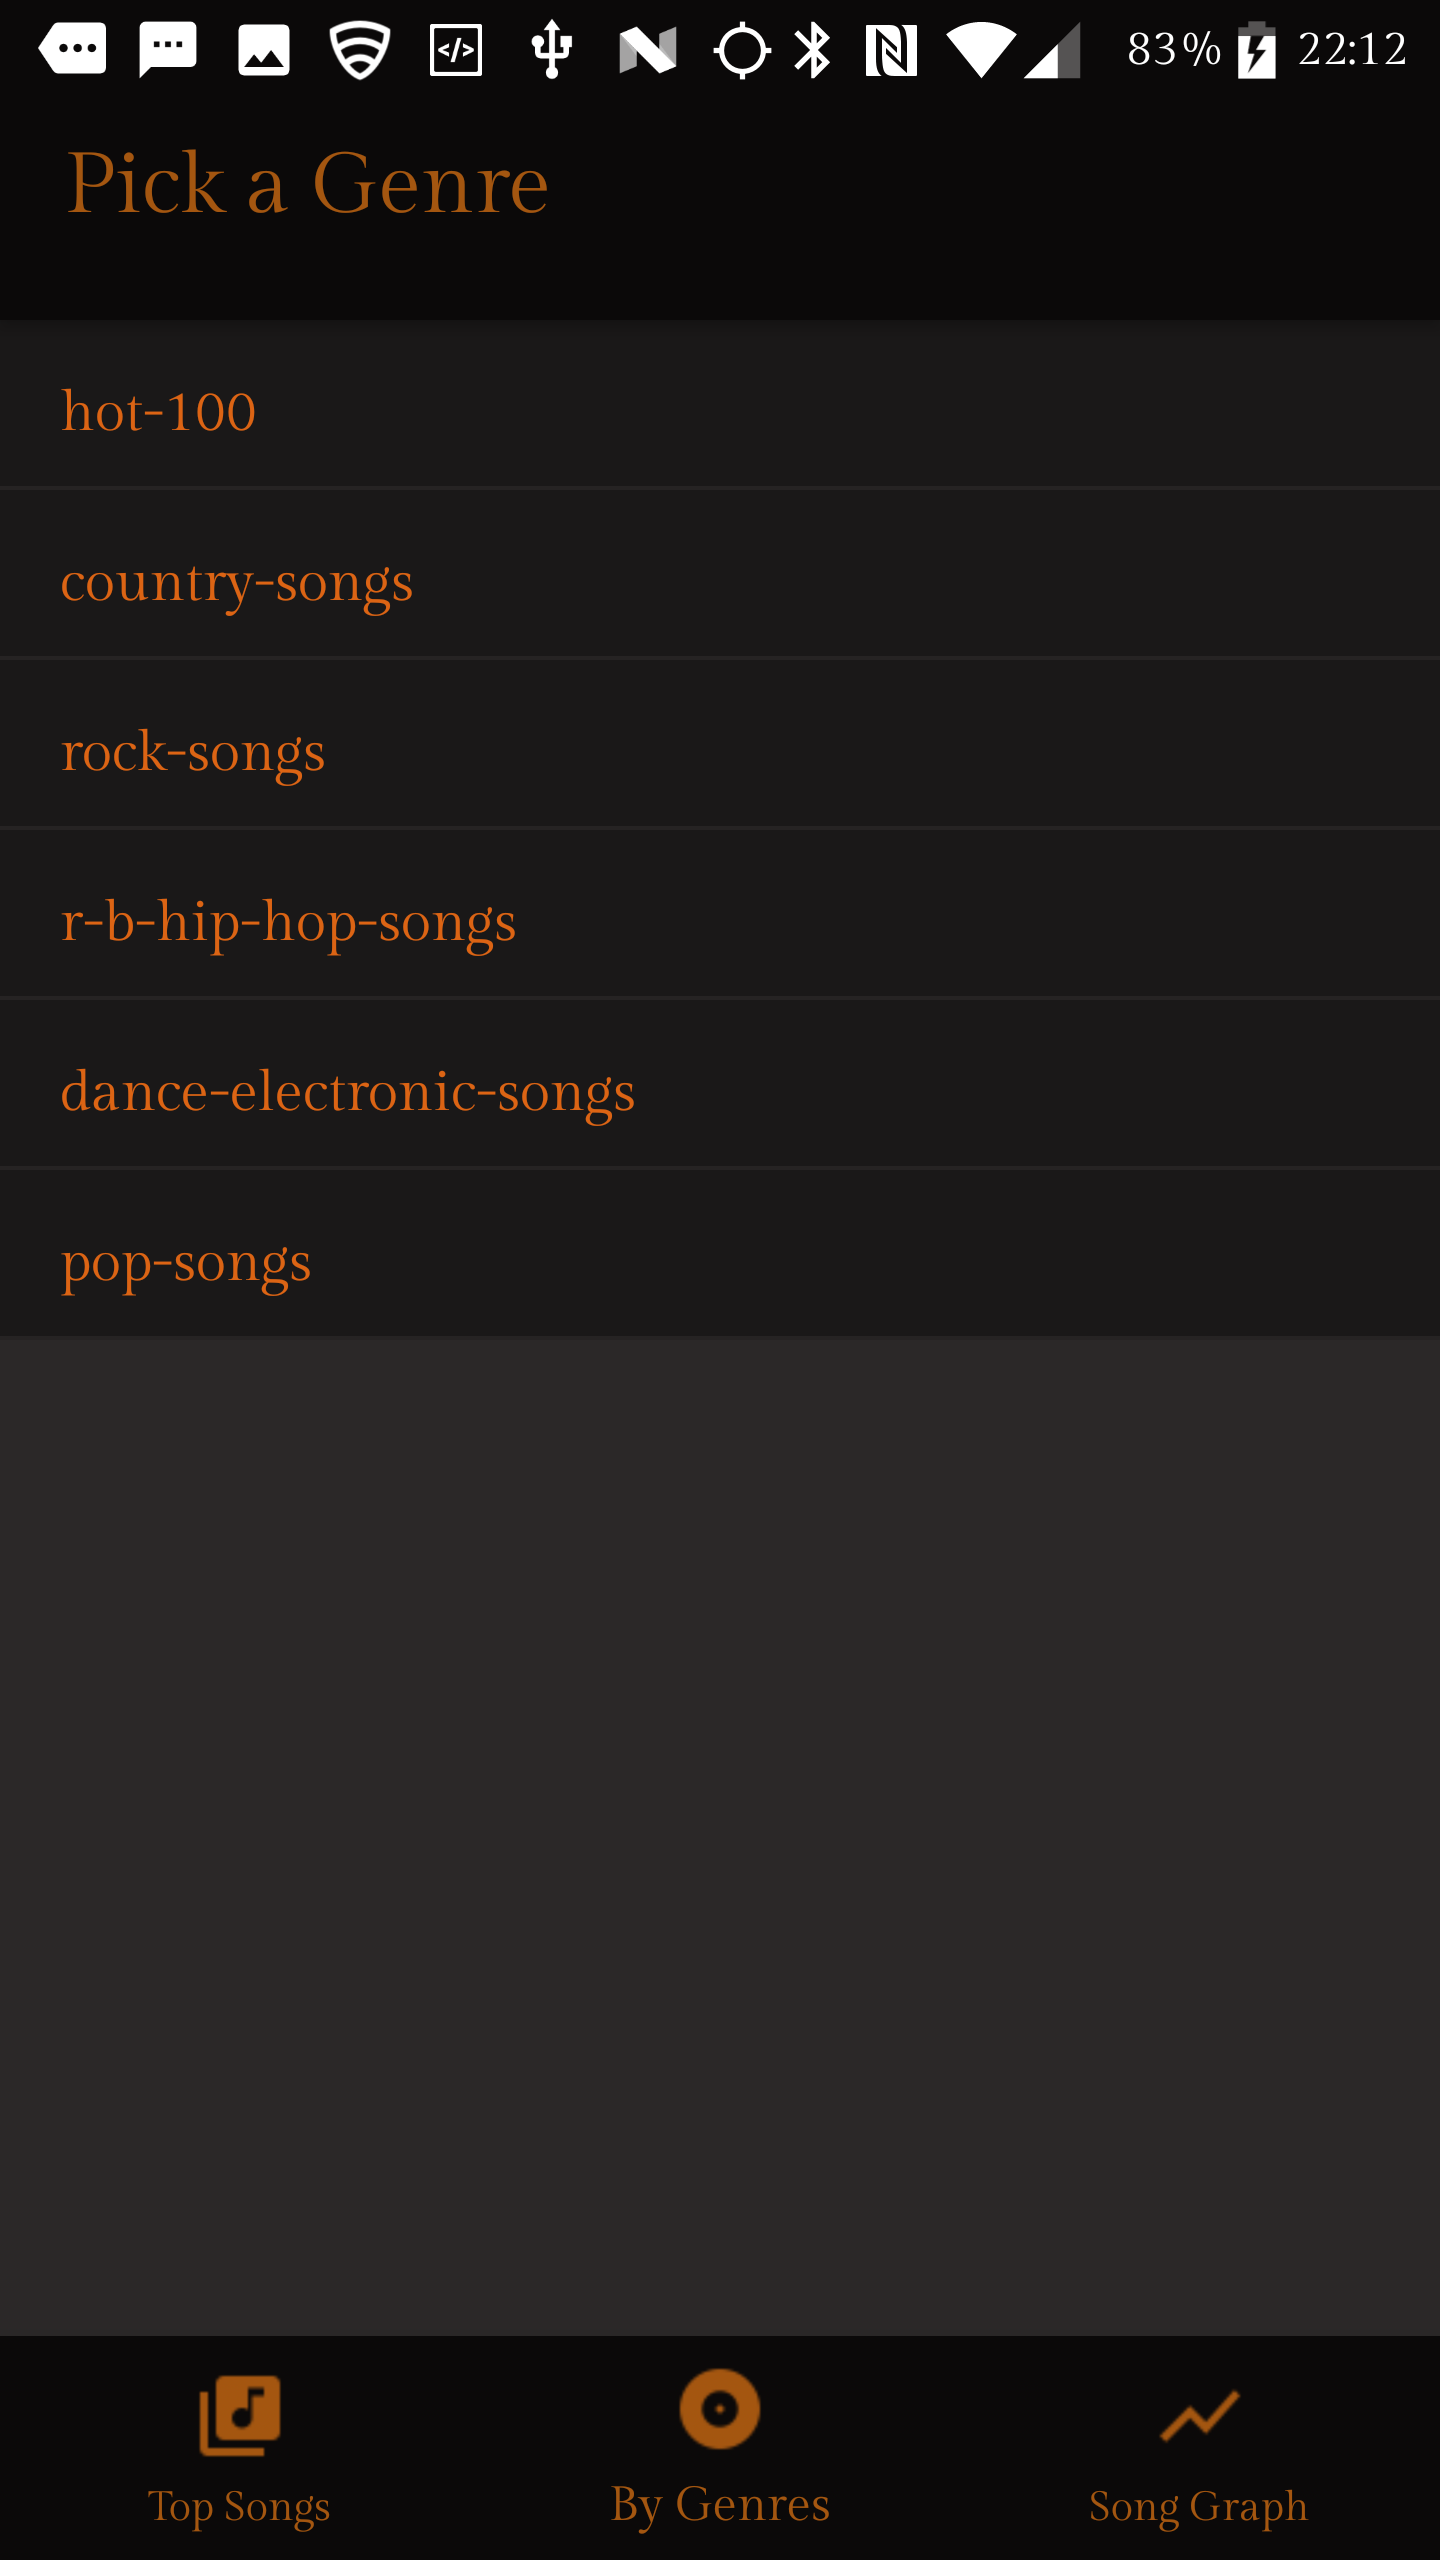
\includegraphics[width=0.75\textwidth]{GenreList.png}
    \caption{Genre Selector}
    \label{label}
  \end{minipage}%
  \begin{minipage}{.5\textwidth}
    \centering
    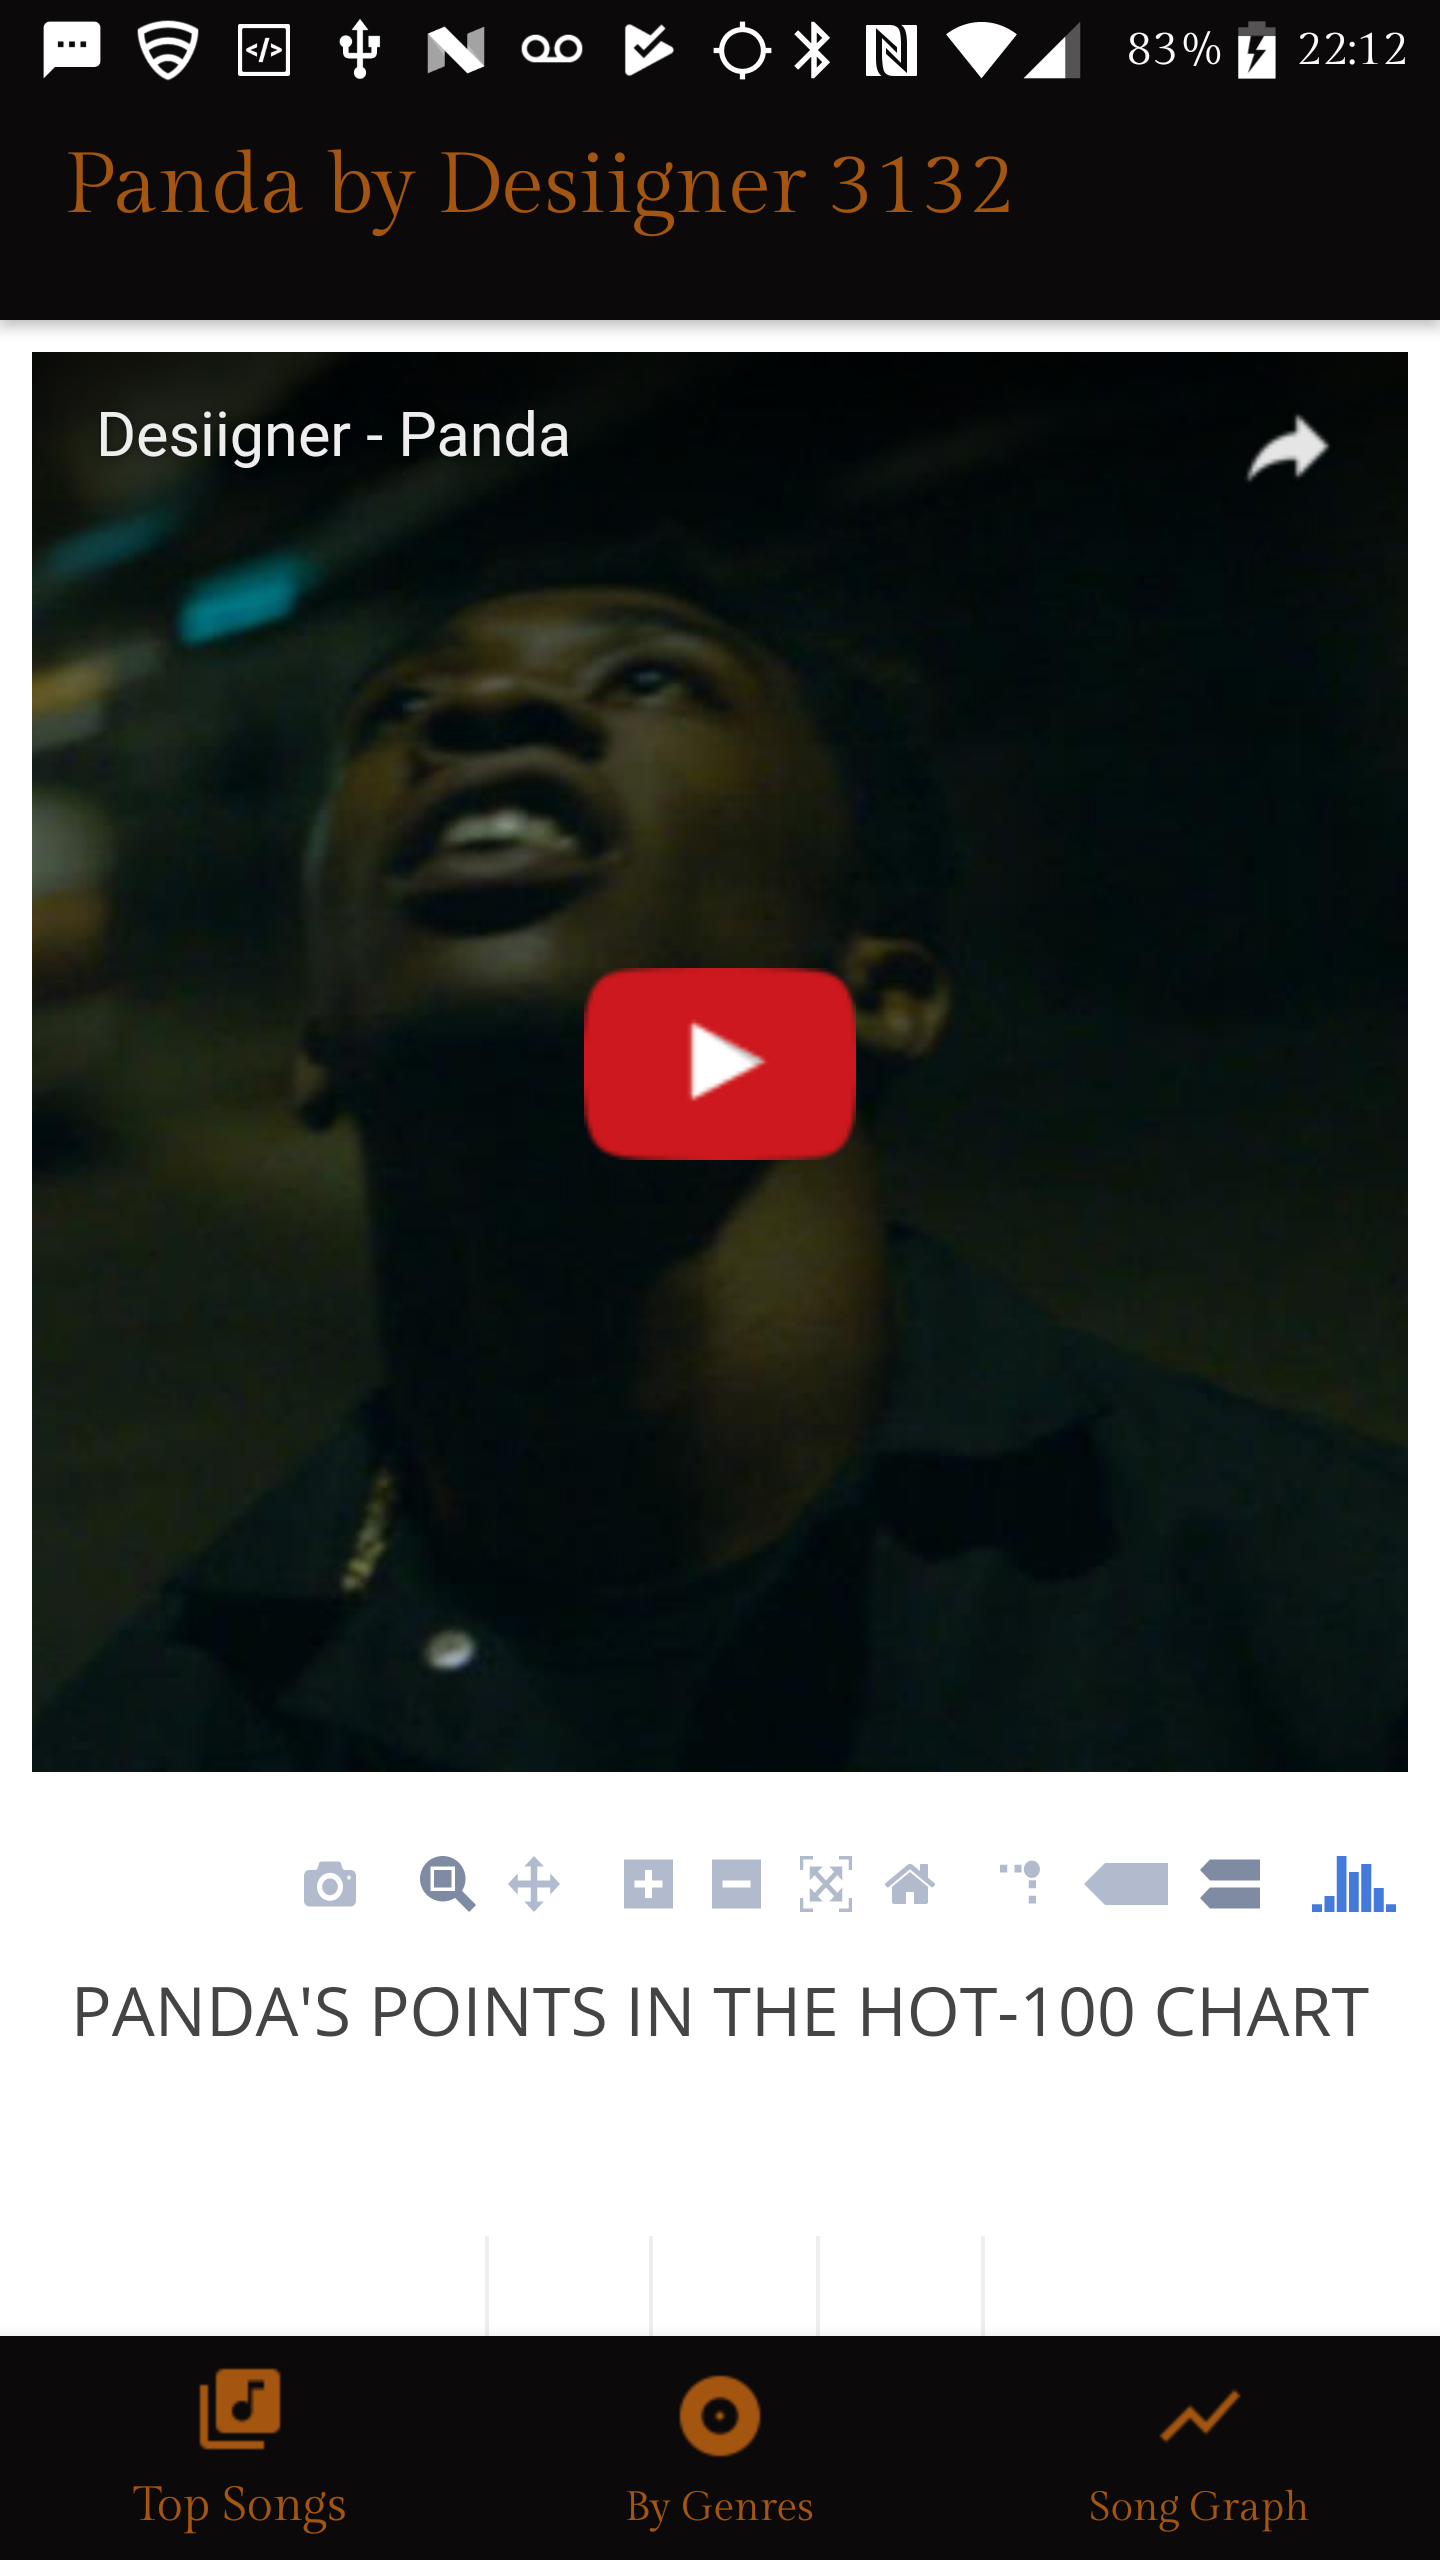
\includegraphics[width=0.75\textwidth]{Video.png}
    \caption{Demo Song Page}
    \label{fig:ER}
  \end{minipage}
\end{figure}


\section*{Implementation Details}
\subsection*{Billboard API}
The Billboard API was rather frustrating to use at times.
Originally we wanted to have a Rap genre within our database, but for some odd reason date incrementation would not work within the Rap genre, so that was scrapped.
Dates in general were rather difficult to work with.
Because the API takes in dates as strings rather than as DateTime objects there was frequent conversions that had to take place between the API and our database itself.
Moreover, the API came packaged with a .next function which was designed to fetch the next week's chart each time it was iterated over.
Unfortunately this functionality proved to not be useful as breaking was consistent.
We opted for timedelta objects for week incrementation in a substitute. 
Moreover, if the chart did not exist on the current date, the API would return a null list.
However, the API does not fetch a chart.date from a null list, which lead to frequent breaking and patching within our dbinit file. 
\subsection*{SQLAlchemy}
In order to effectively use the Billboard API we opted to back end our initial database with python and an init script. SQLAlchemy is a great set of database bindings to use for storing information when using python because it allows for SQL queries to be returned in a Python-like structure which make for an easier implementation and integration into our project overall.
SQLAlchemy's documentation, while extensive, did not quite translate well to our project.
Because of the environment that they placed their documentation in, we were only able to gain a basic understanding of how the system works.
Often, we found ourself reverting to stack overflow posts whenever we found an issue that we needed to solve.
The Flask Mega Tutorial by Miguel Grinberg proved to be vital in getting the setup of our database established, and allowed for us to get the ball rolling.
While it was nice dealing with Python based objects, we have had to recompile our database on multiple occasions due to errors within the base models, and SQLAlchemy's refusal to support migration out of the box.
Additionally, rather than directing to a Firebase within our python script for the initialization, we needed a way to store information to later query. 
The SQLAlchemy structure allowed us to have this delay ability. 
\subsection*{FireBase}
We opted to use FireBase in an effort to support our ability to update the song information over time without asking the users to constantly update through the play store. This gives us a lot of flexibility in regards to future updates only having to push new functionality to the play store. However Firebase did not come without its own set of woes. The official FireBase documentation is terribly deprecated with many referenced classes and methods appearing to not exist at all. This being the case our methods had to be peiced together from solutions to use-cases with varying similarities. Once these initial hurdles were overcome the FireBase was easy to use, reliable and overall a great solution. We believe that storing our content in this way will give us many opportunities to grow our functionality with minimal growing pains.  
\subsection*{Plotly}
Plotly was used for the graphing interface of our website.
When we first acquired this service in 2016 we were promised by the company that we would be allowed to make 10,000 API calls a day.
As it currently stands, our queries have been cut to only one-tenth of our original allotment. While this did hinder our progress, it did not stop us all-together. That being said, in future updates we do doubt that Plotly will continue to be the graphing option of choice.
The reason for its use is to provide off application data storage and image options to not only increase efficiency but also to not clog the app with necessary storage.
\subsection*{JSoup}
JSoup was used for YouTube URL scraping.
As the YouTube API proved to be cumbersome to use, we opted for which we neglected in choosing the Billboard API as mentioned above.
JSoup allowed for our songs to be dynamically linked upon song-request from our Application.
This was not placed into our database due to the volatility of YouTube videos as well as the lack of need, as nothing needs to be rendered unlike plotly.
\subsection*{Andorid Specific Implementation Designs}

\subsubsection*{ListView}
ListViews are being used to allow for simple naviagtion in the lists for top-songs, and genres respectively. Clickable implementation was added for fragment transitions.

\subsubsection*{WebViews}
The WebView is using an embed technique rather than a straight URL to load data. 
This allows for the webview to be more or less static and makes the scroll of the webpage more manageable for the user rther than traditional WebViews,
resulting in the webview not being scrolled, but rather the scrollview that it is encapsulated within.
The WebView is used for the youtube embed links and the graphs. 
They are dynamically added to the fragment rather than statically as anywhere between 2-8 webviews can be used on one song-graph page depending on the individual
song and the number of charts that it made it on. 
\subsubsection*{BottomNaviagtionView}
The bottom naviagtion view is used for the menu layouts to allow for simple navigation bewtween fragments in the main layout.
\subsubsection*{Fragments}
In order to simplify the UI and maintain consistency fragments are used in the main layout rather than individual activities. 

\section*{Future Development}
\subsection*{Artist Integration}
The original concept of the app was to provide not only a top-song list by genre, but also a top-artist list. Due to time constraints as well as FireBase implementation difficulties we only have a top-song data structure enabled. That being said, top-artist structures are not far away. We have the information available and formatted within our SQLAlchemy database as it stands, so the update script can come in the next patch.
\subsection*{Time \& Dates}
In a future instantiation of the app we would like to have time capsule information available: To be able to see who dominated the 90s, 2000s, 80s, or 60s on the charts. As billboard first started producing charts in 1953, we believe that generational information would be fascinating to see. We also want to make the slider dynamic so that the user could determine where they want to see chart domination times. 
\subsection*{Search Terms}
We want to be able to implement a search bar for either Artist or Songs. Again, an easy fix which could be implemented in the next update.  
\subsection*{Firebase Update Scripts}
Moving forward we would like to implement a python script that pulls down new  information from billboard, updates the SQL database and pushes changes to the firebase weekly. So that our users can come back to our app over time and watch out for new trends and follow their favorite songs.
\subsection*{Bottom Naviagtion Button and Scroll Placement}
As of now, our bottom naviagtion view buttons do not work well with our intents or remember your last position within the app. We Intend to fix this in future generations.
\subsection*{Youtube Embedding}
While the youtube links do work, and you can turn off our phone and listen to youtube at the same time, which we think is pretty awesome, it is not perfect as there is an extra step on most videos due to youtube restrictions. We want to find a way around this in future generations and stay away from the google API.
We don't want to be limited by API Calls. We would like to also have an auto next function to almost create a playlist and not have to go back to the songlist to play the next song on said list. 
\subsection*{Graphs}
The Graph layout highly contrasts our dark view, we need to recolor them, but actually did run out of time to do this.
Additionally we did at first believe that tick marks would crowd the page, and they do on the plot.ly page, but in the mobile program, we do feel that they are warranted, and without them the user does get confused.
We will be adding them back in our next installment. 







\begin{thebibliography}{00}
\bibitem{1}
www.billboard.com
\bibitem{2}
www.github.com/guoguo12/billboard-charts
\bibitem{3}
https://blog.miguelgrinberg.com/post/the-flask-mega-tutorial-part-i-hello-world
\bibitem{4}
https://firebase.google.com/
\bibitem{5}
https://plot.ly/python/axes/
\end{thebibliography}

\end{document}
